\chapter{appendix}\label{chapter:appendixA}


\section{Hidden Markov Model}
%TODO: Hidden Markov Model  


\chapter{Figures}\label{chapter:appendixB}

\section{Stability analyze of our model}
This section demonstrates the stability of our proposed model, which is adapted from JODIE as discussed in Chapter~\ref{chapter:methodology}. We ran the model five times on each dynamic graph, as well as on the combined graphs, and present the results in Figures~\ref{fig:all_results1} and \ref{fig:all_results2}.

In these figures, the blue bars represent the AUROC scores of predictions for the old nodes, while the red bars represent the AUROC scores of predictions for the new nodes. The two parallel horizontal lines correspond to the average AUROC scores for the old nodes and new nodes, respectively, and are color-coded accordingly.

From the results, it is evident that in the majority of cases, there are no significant differences across the different runs when training on the same dynamic graph. This observation is particularly clear when the AUROC scores are relatively high, around 0.8. This consistency across multiple runs provides strong evidence that our model exhibits stability and that the obtained results are reliable.

% TODO: illustrate the following graphs
\begin{figure}
    \centering
    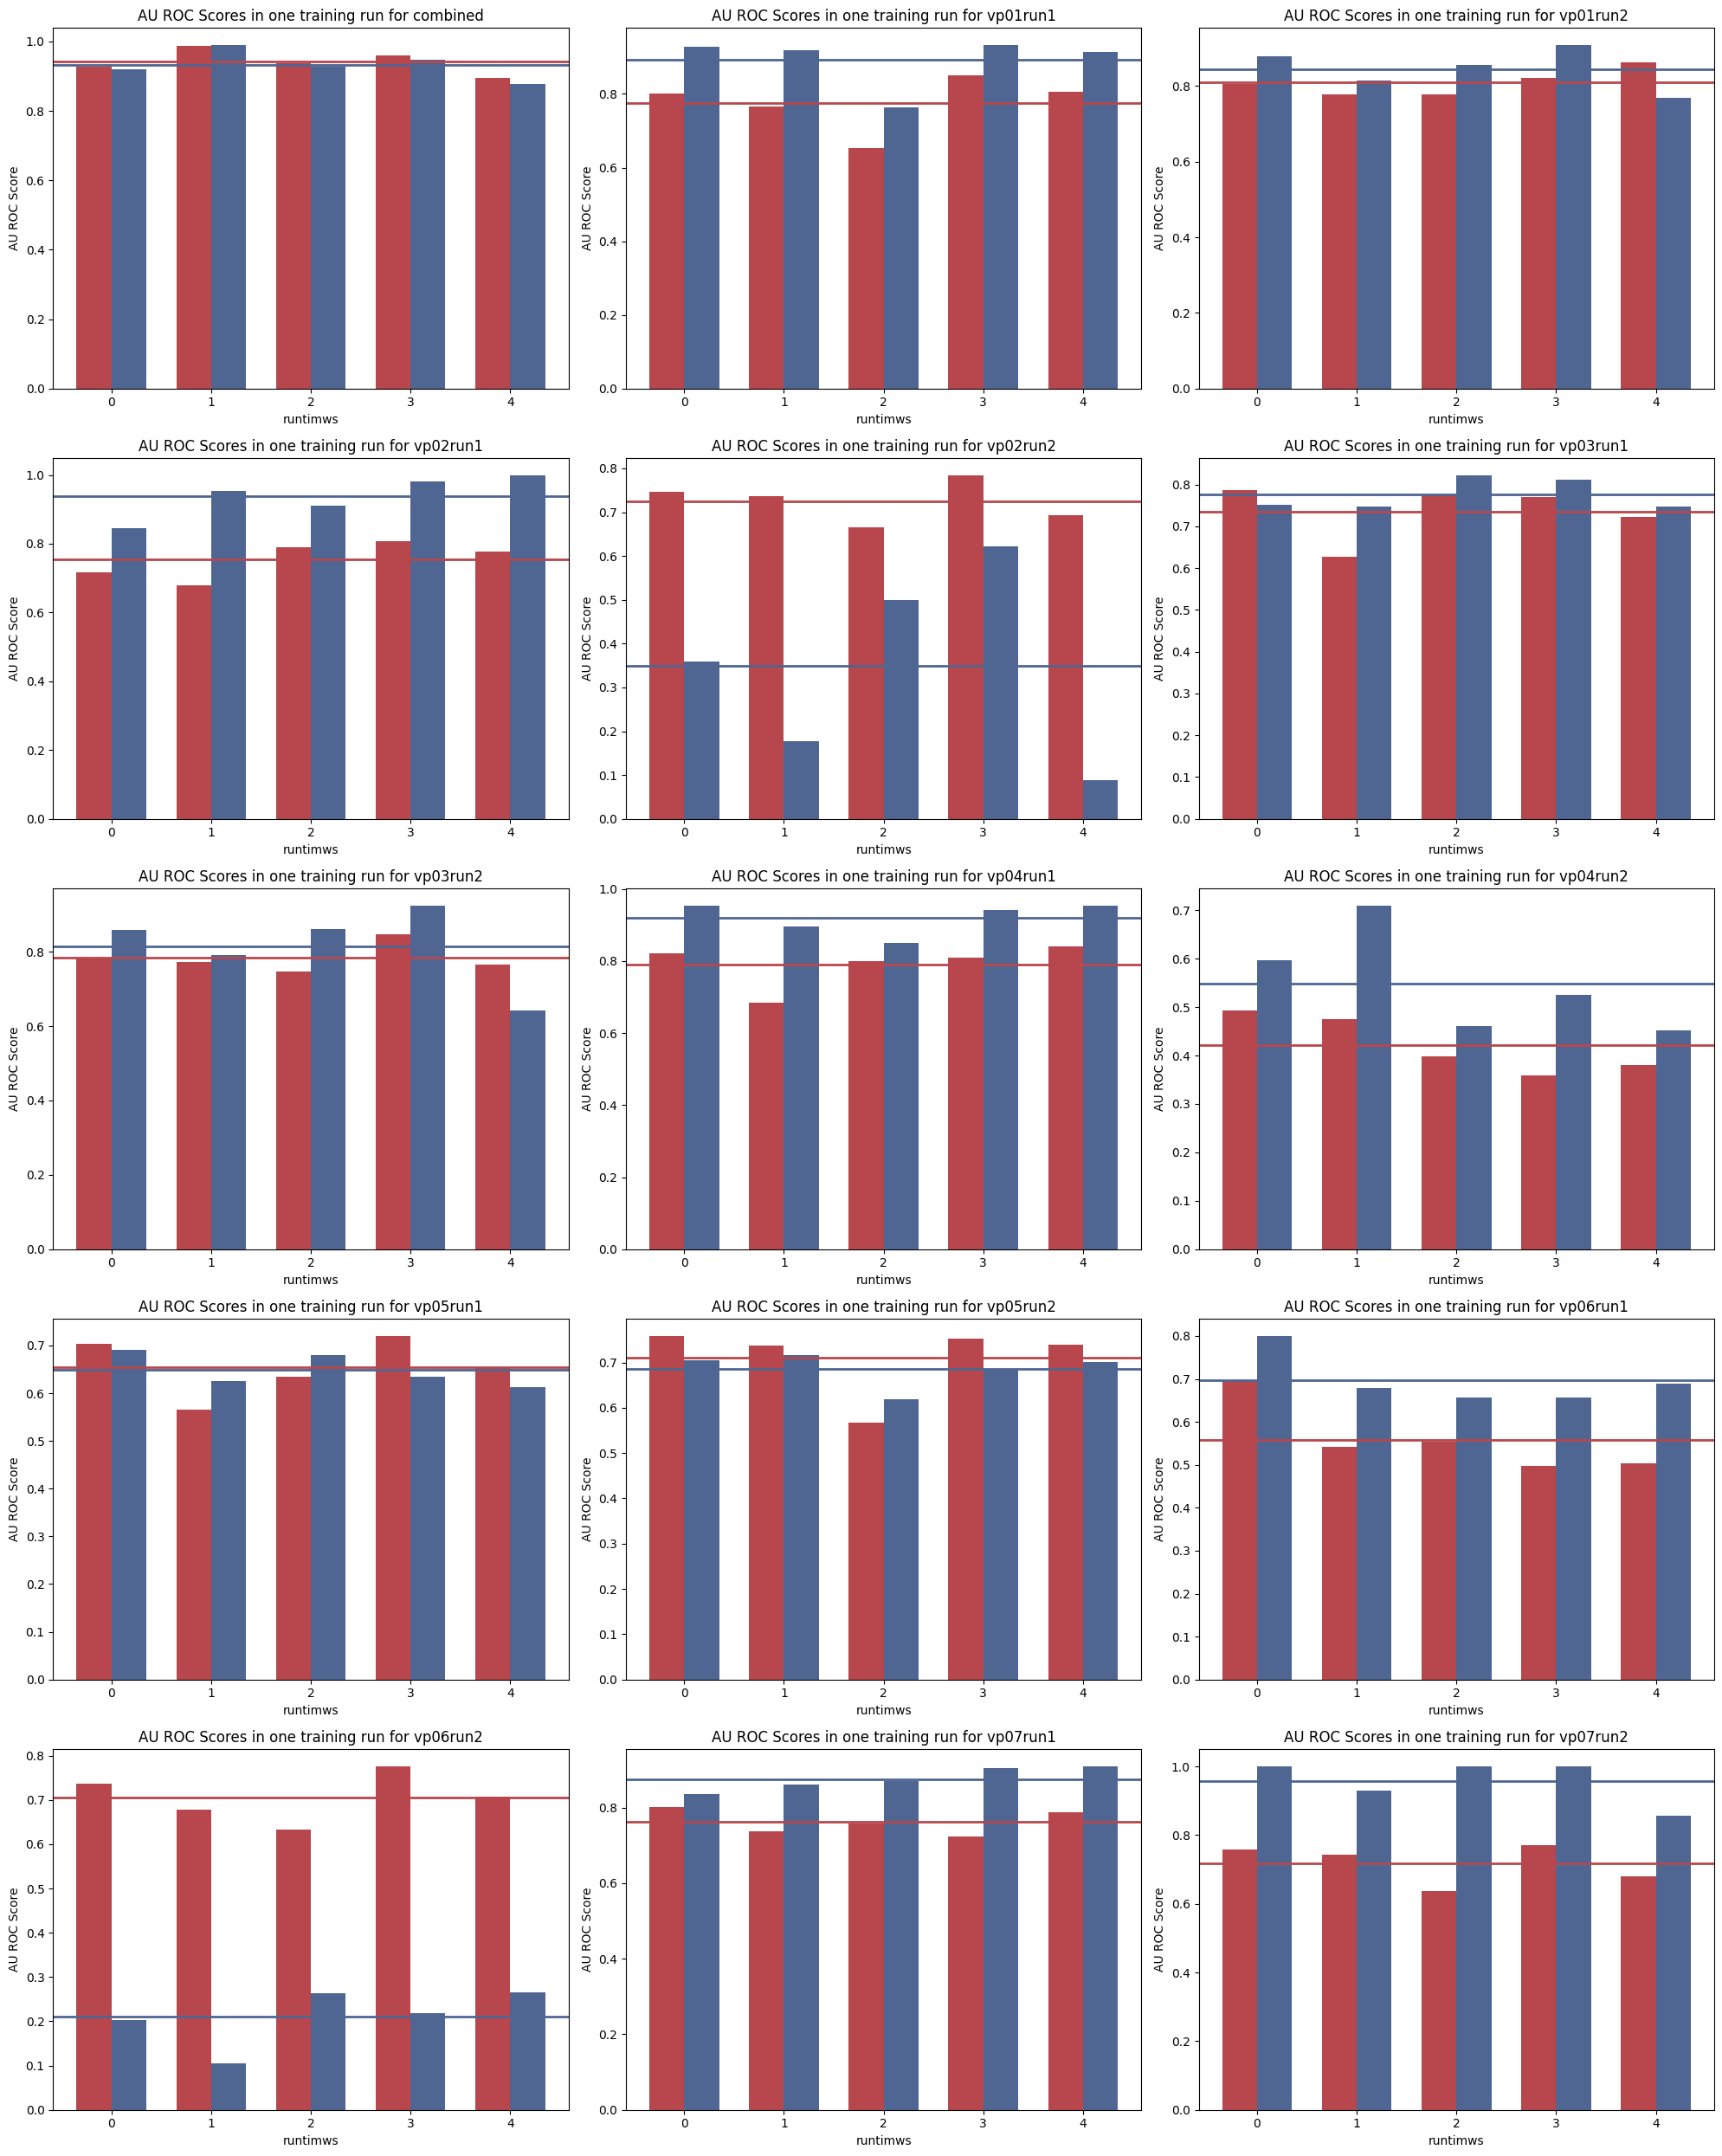
\includegraphics[width=\textwidth]{figures/05_all_results1.png}
    \caption{all the results of the model JODIE with state embedding-1} 
    \label{fig:all_results1}
\end{figure}

\begin{figure}
    \centering
    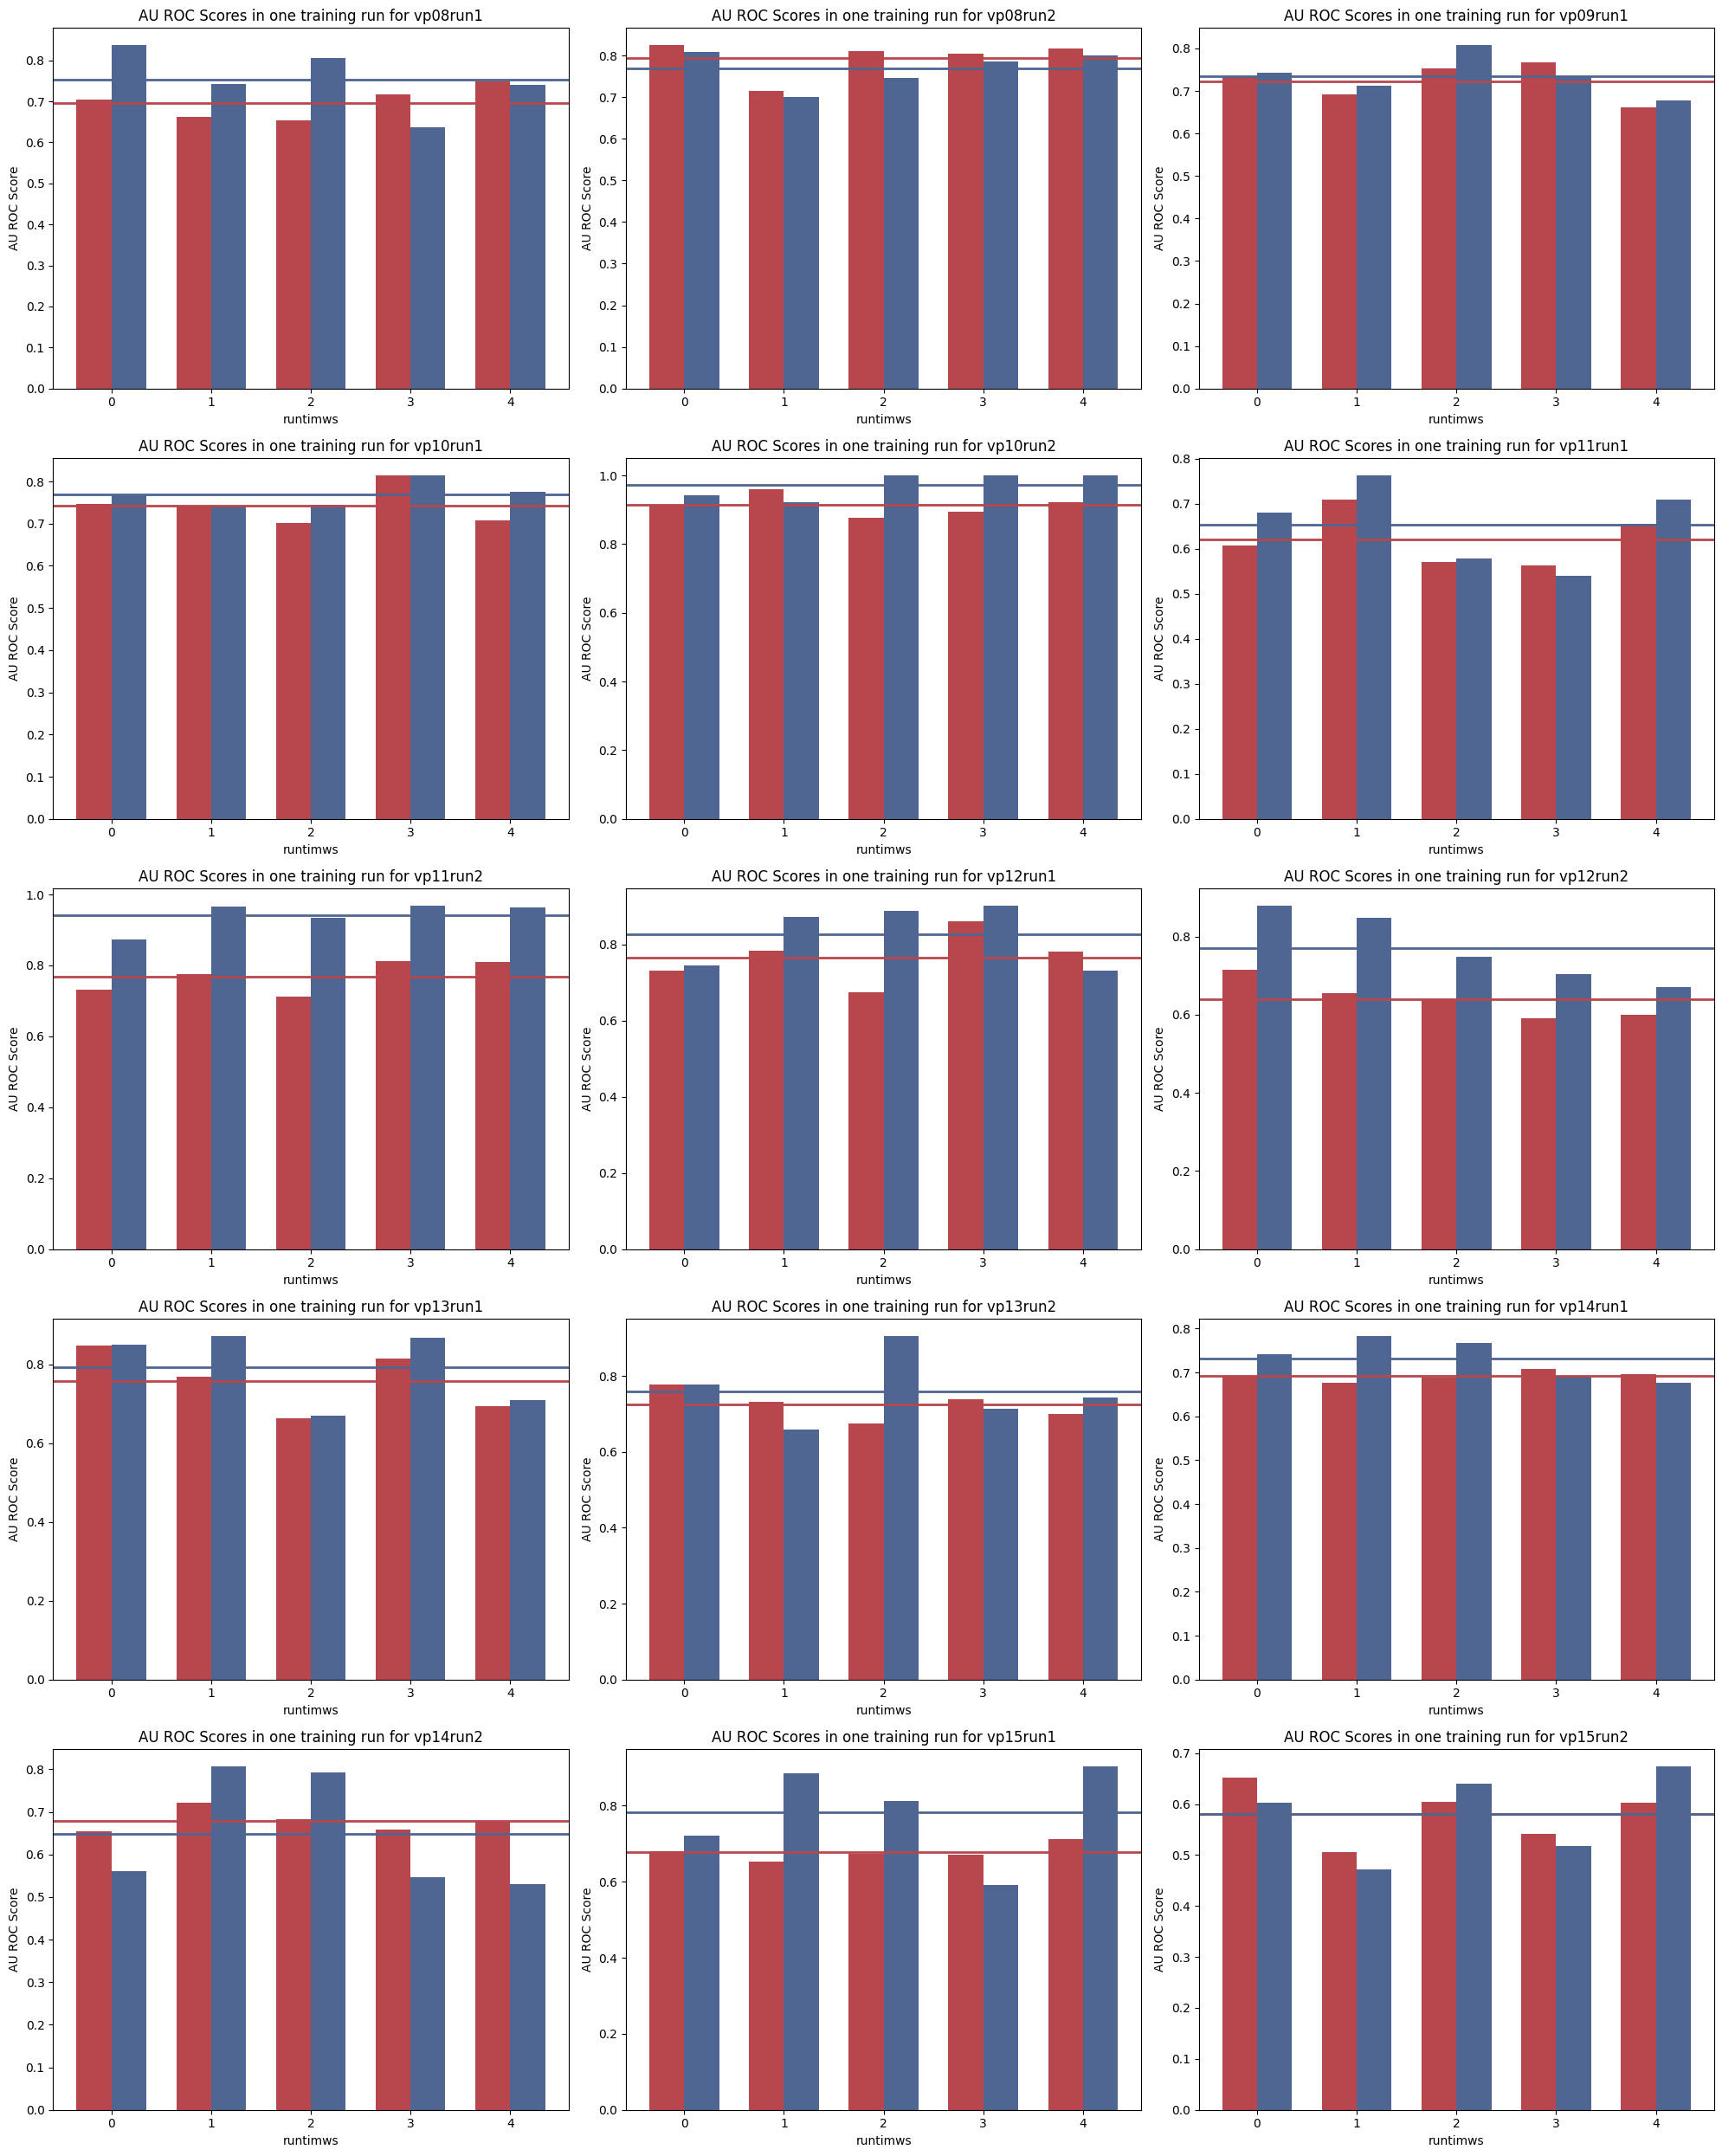
\includegraphics[width=\textwidth]{figures/05_all_results2.png}
    \caption{all the results of the model JODIE with state embedding-2} 
    \label{fig:all_results2}
\end{figure}
